\section{State of the art in ESD testing}

To ensure proper operation once in the field, hardware is tested against \gls{esd} using different test methods and standards.
The goal for each method is to reproduce a particular \gls{esd} waveform in lab conditions.
In this chapter, we will introduce most relevant \gls{esd} generators, which will be useful later on for modeling them accurately.

\subsection{Transmission Line Pulsing (TLP)}

\gls{tlp} generators use the discharge of a coaxial cable to generate a fast and square pulse.
The cable is charged by a high-voltage power supply then discharged into a load by switching a relay.

\begin{figure}[h]
  \centering
  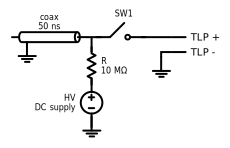
\includegraphics{src/1/figures/tlp_concept.pdf}
  \caption{Minimal example of a \gls{tlp} system}
  \label{tlp_concept}
\end{figure}

The charge is performed through a high value resistor to keep the current small and avoid generating oscillations on the cable.

TLP systems constitute very well-controlled test generators, because the pulse is generated inside a shielded and isolated environment.
Characteristic impedance can be controlled up to the load.
Those features allow for extremely clean and repeatable pulse waveforms.

\begin{figure}[h]
  \centering
  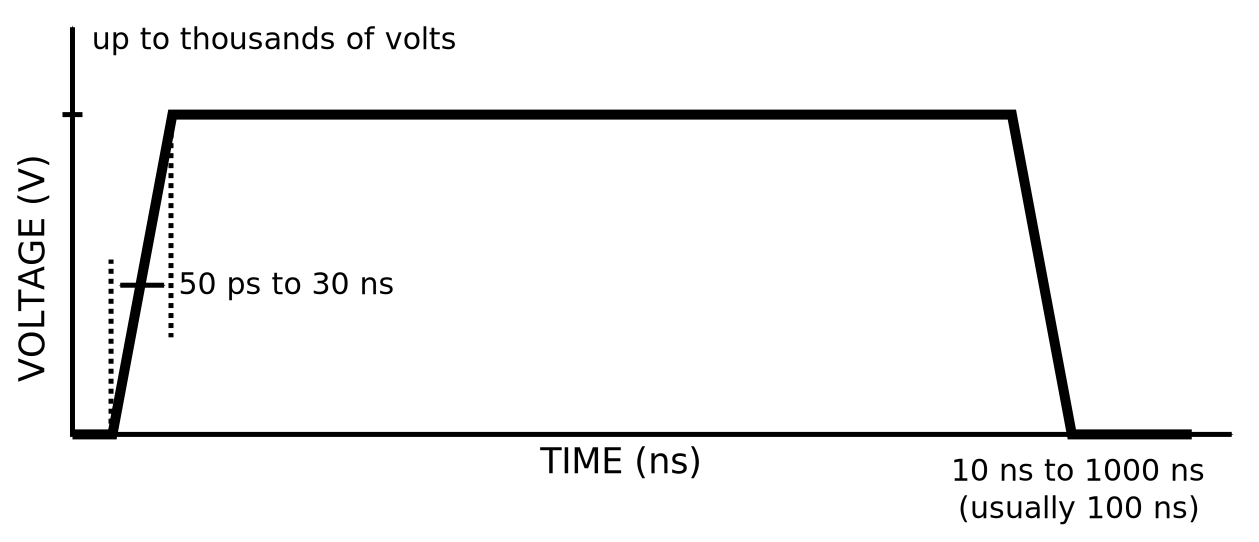
\includegraphics[width=\textwidth]{src/1/figures/tlp_pulse.pdf}
  \caption{Main characteristics of a \gls{tlp} pulse on a resistive load}
  \label{tlp_pulse}
\end{figure}

Using time-domain reflectometry methods, it is possible to reconstitute the current and voltage waveforms inside the load,
from measured current and voltage inside the \gls{tlp}, even if the \gls{tlp} and the load are separated by cables, devices, etc.
Indeed, the superposition of the incident and reflected pulses during the discharge show that the voltage and current
measured inside the generator are direct image of the ones accross and through the load.

\gls{tlp} are extensively used for characterizing the response of ESD protections \cite{TLP, TLPforESDProtectionCz}
or testing the response of systems and devices against a clean and well repeatable pulse \cite{TLPthroubleshooting, LacrampeTransientImmunity}.

\subsection{ESD Gun (IEC 61000-4-2 / ISO 10605)}
blabla

\subsection{ISO 7637-2}

\subsection{Burst test (IEC 61000-4-4)}

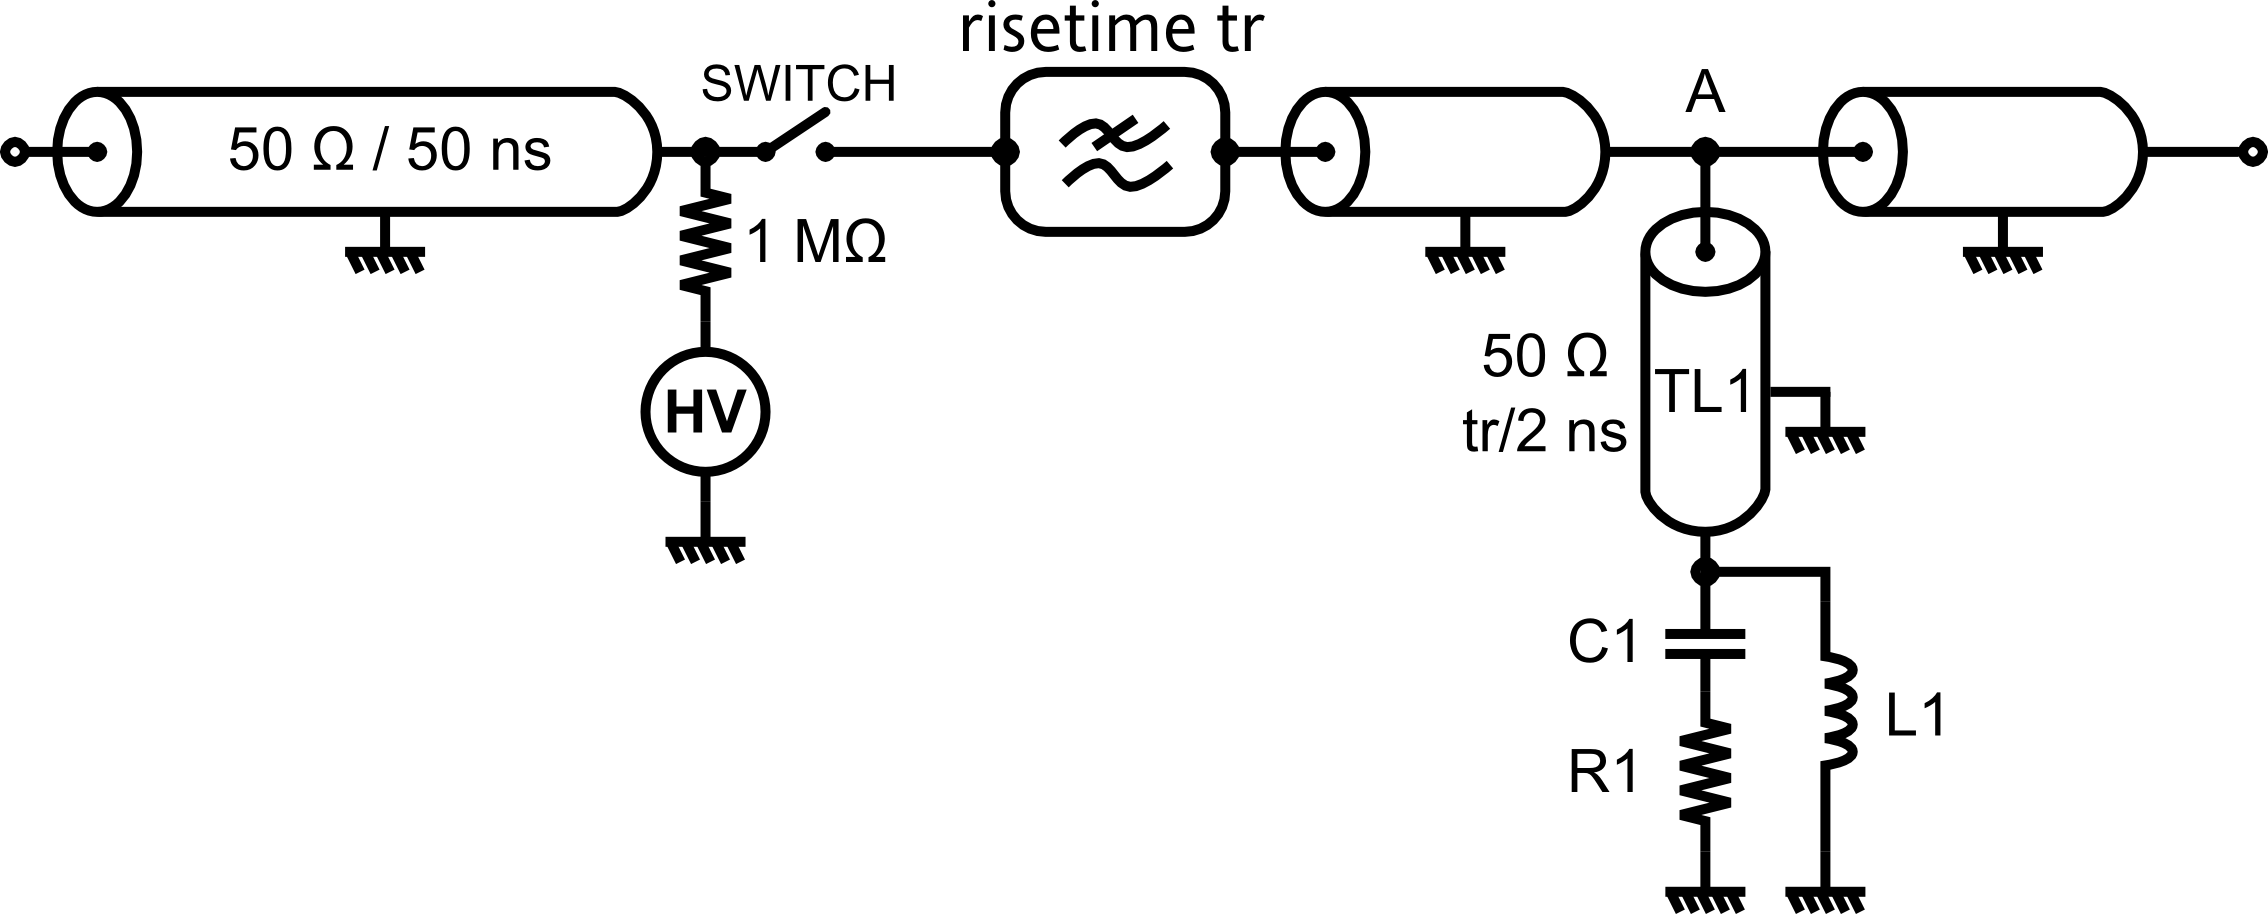
\includegraphics[width=\textwidth,height=\textheight,keepaspectratio]{src/2/figures/tlp_iec.png}
